\documentclass{book}
\usepackage{pgfplots}
\usepackage{imakeidx}
\usepackage{amsfonts}
\usepackage{amsthm}
\usepackage{tikz}
\usepackage{array}
\usepackage{imakeidx}
\newcommand{\SectionBreak}{%
    %\vskip 0.5ex

    \nointerlineskip
    \moveright 0.125\textwidth \vbox{\hrule width0.75\textwidth}
    \nointerlineskip
    %\vskip 0.5ex
    \makeatletter
        %\@afterindenfalse%
    \makeatother

}

\newtheorem{definition}{Definizione}

\pgfplotsset{compat=1.18}


\author{F. Piazza \and G. Michieletto}
\title{%
	Appunti di Analisi Matematica II \\
	\large corso della prof.ssa B.Noris \\
	Politecnico di Milano\\
	\bigskip
	\bigskip

	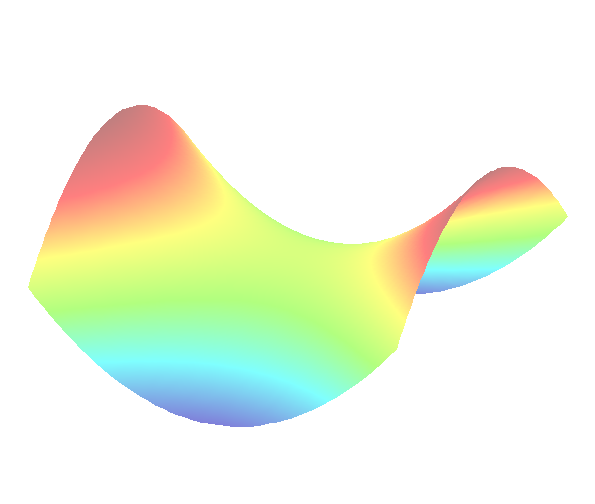
\begin{tikzpicture}
	\begin{axis}[axis line style={draw=none}, colormap/bluered]
	\pgfplotsset{ticks=none}
	% \addplot [domain=0:1, samples=100, color=black, thick] {x};
	\addplot3[surf, samples=50, opacity=0.5, shader=interp] {x^2-y^2};
	\end{axis}
	\end{tikzpicture}
}


\begin{document}


\maketitle

\chapter{Equazioni differenziali}
\section{Equazioni differenziali del 1° ordine}
\begin{definition}
	Una equazione differenziale o \emph{EDO} del 1° ordine è una relazione tra una funzione $y$ e la sua derivata $y'$ che può essere scritta come
	\begin{equation}
		y' = f(y)
	\end{equation}
	dove $f$ è una funzione continua su un intervallo $I\subseteq\mathbb{R}$.
\end{definition}

Esempi:
\begin{itemize}
	\item \emph{Tema d'esame gennaio 2021}\\$y' = t \sqrt{y_{(t^2)}+1}$ è in forma normale con $f(t,s) = t \sqrt{s^2+1}$. Il dominio di $f$ è $I = \mathbb{R} \times \mathbb{R} = \mathbb{R}^2$.
	\item $y'_{(t)} = \frac{1}{t}$ con $t>0$ diventa $f(t,s) = \frac{1}{t}$. \textbf{Oss:} $f$ non dipende esplicitamente da $s$. \\ Il dominio di $f$ è $\{(t,s) \in \mathbb{R}^2 : s\in\mathbb{R}, t\in\mathbb{R}^* \}$, dunque è diviso in due parti.
			Dovrò quindi risolvere la EDO separatamente nelle due regioni.
			$$ \left\{\begin{array}{lr} y'(0)=\frac{1}{t},	t>0 \Rightarrow y(t) = ln(t)+c\\ y'(0)=\frac{1}{t},	t<0 \Rightarrow y(t) = ln(-t)+c \end{array}\right. $$
\end{itemize}
\SectionBreak
\begin{definition}
	Si chiama \emph{integrale generale} l'insieme delle soluzioni.
\end{definition}
\begin{definition}
	Si chiama \emph{soluzione particolare} una specifica soluzione.
\end{definition}
\noindent{Una EDO del 1° ordine ha $\infty^1$, soluzioni, cioè avrà una costante arbitraria. In modo analogo, una EDO del 2° ordine avrà $\infty^2$ soluzioni, cioè avrà due costanti arbitrarie.}
Esempi:
\begin{itemize}
	\item integrale generale $ce^t$ con $c$ costante arbitraria. Esempi di soluzioni particolari: $e^t$, $2e^t$, $-e^t$.
	\item $z_{(t)} = -1 + arctan(t)$ con $t\in\mathbb{R}^*$. Esempio di soluzione: $z' = 0 + \frac{1}{1+t^2}$.
\end{itemize}
\textbf{Oss:} La EDO $y'_{(t)} = f(t,y_{(t)})$ è definita per $(t,y)\in dom(f)$

\subsection*{Soluzioni costanti di EDO del 1° ordine}
\begin{definition}
	Una soluzione costante di una EDO del 1° ordine è una funzione $y(t)$ che sia soluzione.
\end{definition}
Quando $y(t)=c$ è soluzione? Sostituisco $c$ a $y$:
\begin{equation}
	y'(t) = f(t,y(t)) \forall t
\end{equation}

Quindi \underline{le soluzioni costanti sono} $y(t) = c$ \underline{con $c$ tale che} $f(t,c) = 0 \forall t$.\\

Esempi:
\begin{itemize}
	\item Eq. Logistica: $y'(t) = ky(t)-hy^2(t)$\\
			$f(t,y)=ky-hy^2$\\
			$f(t,c)= 0 \forall t$ \quad $ky-hy^2=0=y(k-hy)$\\
			Soluzioni costanti: $y=0$ o $y=\frac{k}{h}$
	\item $y'(t)=te^{y(t)}$ \quad $te^{y(t)}=0$ non ha soluzione.
\end{itemize}

\SectionBreak

\subsection*{EDO a variabili separabili}
\begin{definition}
	Una EDO del 1° ordine è detta \emph{a variabili separabili} se è del tipo
	\begin{equation}
		y' = f(t)\cdot g(y(t))
	\end{equation}
	dove $f$ e $g$ sono funzioni continue su intervalli $J_1,J_2\subseteq\mathbb{R}$.
\end{definition}

\begin{center}
	
\textbf{Da integrare con gli appunti della professoressa.\\Lezione del 14/09/2022}

\end{center}



\SectionBreak
\subsection*{Problema di Cauchy}
\begin{definition}
	Data una EDO del 1° ordine $y'_{(t)} = f(t,y_{(t)})$ sia $(t_{0}, y_{0})$ dove la EDO è definita.
	Cioè $(t_{0},y_{0})\in dom(f)$ \\
	Si chiama \emph{problema di Cauchy} il problema di determinare $y : I\subseteq \mathbb{R} \to \mathbb{R}$ che soddisfa:
	$$ \left\{\begin{array}{lr}y'(t)=f(t,y(t)) \\ y(t_{0})=y_{0}\end{array}\right. $$
\end{definition}
Nota: il sistema ha una condizione perché è del 1° ordine. La condizione trova la soluzione particolare che passa per $(t_{0},y_{0})$.\\
\SectionBreak
\subsection*{Come si risolve?}
Step:
\begin{enumerate}
	\item Trova l'integrale generale. ($\infty^1$ soluzioni dipendenti da 1 parametro)
	\item Impongo la condizione $y(t_{0})=y_{0}$ e la costante $c$
	\item Sostituisco $c$ in 1.
\end{enumerate}

\subsubsection*{Esempi}
Aggiungi Esempi\\
\SectionBreak

\subsection*{EDO 1° ordine lineari}
\begin{definition}
	Una EDO del 1° ordine lineare in forma normale è:\\
	\begin{equation}
		y'_{(t)} = a(t)y_{(t)} + b(t)
	\end{equation}
	dove $a$ e $b$ sono funzioni continue su un intervallo $J$ di $\mathbb{R}$.\\
	\textbf{N.B.} $J$ è il più grande intervallo di $\mathbb{R}$ tale che $a,b\in J$.\\
\end{definition}

\begin{definition}
	Si chiama EDO omogenea associata
	\begin{equation}
		y'_{(t)} = a(t)y_{(t)}\\
	\end{equation}
\end{definition}
Esempio:\\
Aggiungi esempi
\\
\SectionBreak
\subsection*{Principio di sovrapposizione}
Sia $a: J\subseteq\mathbb{R} \to \mathbb{R}$ una funzione continua su $J$.\\L'applicazione $\mathcal{L}(y)=y'-a(t)\cdot y$ è lineare.\medskip\\
Più esplicitamente, dati $c_1,c_2 \in \mathbb{R}$:\\
$\mathcal{L}(c_1y_1+c_2y_2)=c_1\mathcal{L}(y_1)+c_2\mathcal{L}(y_2) \forall y_1,y_2$ funzioni derivabili.\medskip\\
Ancora più esplicitamente:
se $\mathcal{L}(y_1)=b_1$ cioè $y'_1=a(t)y_1+b_1$\\
se $\mathcal{L}(y_2)=b_2$ cioè $y'_2=a(t)y_2+b_2$\\
allora $\mathcal{L}(c_1y_1+c_2y_2)=c_1b_1+c_2b_2$ cioè $y'_{(t)}=a(t)(c_1y_1+c_2y_2)+c_1b_1+c_2b_2$\\
cioè $(c_1y_1+c_2y_2)'=a(t)(c_1y_1+c_2y_2)+c_1b_1+c_2b_2$\\
\textbf{Oss:} \begin{itemize}
	\item Prendo due soluzioni distinde della EDO 
    \item  $y'=a(t)y + b(t)$\\
\end{itemize}
\SectionBreak
\subsection*{Esistenza e unicità globale di Cauchy}
Siano $J\subseteq\mathbb{R}$ intervallo e $a,b: J\to \mathbb{R}$ continue.\\
Per ogni $t_0\in J, y_0 \in \mathbb{R}$ il problema di Cauchy:
\begin{equation}
	\left\{\begin{array}{lr}y'(t)=a(t)y(t)+b(t) \\ y(t_0)=y_0\end{array}\right.
\end{equation}
ha una soluzione unica $y: J\to \mathbb{R}$ definita su $J$.\\
\textbf{Aggiungi parte in blu lezione 16/09/2022}\\

\SectionBreak

\subsection*{Teorema Formula risolutiva per EDO lineari 1° ordine}
$a,b: J\subseteq\mathbb{R}\to\mathbb{R}$ \quad $y'(t) = a(t)y(t)+b(t)$\\
L'integrale generale è dato dalla formula:
\begin{equation}
	y(t)=e^{A(t)}+\left( \int e^{-A(x)}b(x)dx + c \right) \quad \forall c\in \mathbb{R}
\end{equation}
dove $A(t)$ è una primitiva di $a$.\\

\emph{\textbf{Dim. 1 - da sapere all'esame}}\\
\begin{itemize}
	\item Porto $ay$ sulla sinistra\\
			$y'-ay=b$
	\item Moltiplico l'equazione per $e^{-A}$\\
			$e^{-A}y'-e^{-A}ay=e^{-A}b$
	\item Riconosco\\
			$y'(t)e^{-A(t)}-a(t)y(t)e^{-A(t)}=\left(y(t)e^{-A(t)}\right)$\\
			Quindi la EDO iniziale si riscrive equivalentemente:\\
			$(ye^{-A})'=be^{-A}$
	\item Integro\\
			$y(t)e^{-A(t)}=\int be^{-A(t)}dt+c$
	\item Moltiplico tutto per $e^{A(t)}$\\
			$y(t)=e^{A(t)}\left(\int be^{-A(t)}dt+c\right)$
\end{itemize}

\SectionBreak

\subsection*{Equazione di Bernoulli}
\begin{definition}
	Si chiamano \emph{equazione di Bernoulli} le EDO del 1° ordine lineari di forma:\\
	\begin{equation}
		y'_{(t)} = k(t)y_{(t)} + h(t)y_{(t)}^\alpha \quad \forall \alpha \in \mathbb{R}\setminus \{0,1\}
	\end{equation}
	con $k,y: J\subseteq\mathbb{R}\to\mathbb{R}$ continue.
\end{definition}

\textbf{Premesse:}\\
\begin{enumerate}
	\item Per semplificare ci occupiamo solo di soluzioni $y \geq 0$
	\item nel caso $\alpha<1$ accadono fenomeni strani, però la tecnica risolutiva è comunque valida
\end{enumerate}

\noindent{Procedimento di risoluzione:}\\
\begin{enumerate}
	\item Cerchiamo le soluzioni costanti (c'è sempre almeno quella nulla)
	\item divido per $y^\alpha$\\
			$y'(t) = k(t)y(t) + h(t)$\\
			$y'(t) = k(t)y(t)^{1-\alpha} + h(t)$
	\item Pongo $z(t)=y(t)^{1-\alpha}$\\
			Quale è l'equazione soddisfatta da $z$?\\
			$z'(t)= \left(1-\alpha\right)\left[k(t)y(t)^{1-\alpha}+h(t)\right] $\\
			$z'(t)=\left(1-\alpha\right)k(t)z(t)+\left(1-\alpha\right)h(t)$\\
	\item Risolvo l'equazione lineare in $z$
	\item Torno alla variabile $y = z(t)^{\frac{1}{1-\alpha}}$
\end{enumerate}

\SectionBreak

\subsection*{Equazione Logistica}
$y(t) = $ numero di individui infetti al tempo $t$\\
$y: J\subseteq\mathbb{R}^+\to\mathbb{R}^+$
\bigskip\\
\textbf{1° Modello: Malthus (inizio '800)}\\
Il tasso di crescita della popolazione è proporzionale alla popolazione stessa.\\
\begin{equation}
	y'(t) = ky(t)
\end{equation}
dove $k\in\mathbb{R}^+$ è la \emph{tasso di crescita} e $k$ è il coefficiente di proporzionalità, dato dalla differenza tra tasso di natalità e tasso di mortalità.\\
integrale generale:
	$y(t) = y(0)e^{kt} $con$ c>0$\\


\textbf{2° Modello: Verhulst (metà '800)}\\
\begin{equation}
	y'(t)=ky(t)-hy(t)^2 \quad  \textnormal{con } k,h > 0
\end{equation}

Il modello prende anche in considerazione la competizione per le risorse al crescere della popolazione.\\
\bigskip
\emph{Simulazione numerica per $k=h=1$}

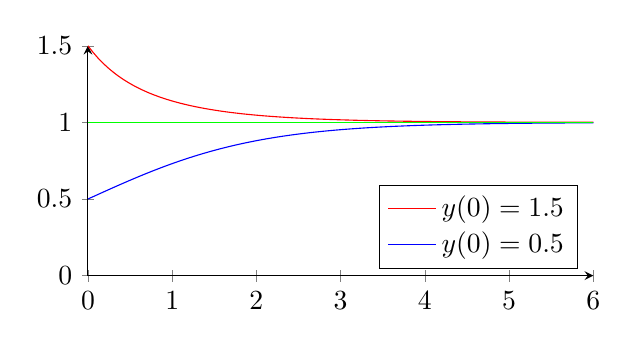
\begin{tikzpicture}
	\begin{axis}[ymin = 0, ymax = 1.5, axis lines = left, height = 4.5cm, width = 8cm, legend pos = south east]

\addplot [
    domain=0:6, 
    samples=100, 
    color=red,
]
{1/(1-(1/3)*e^(-x))};
\addlegendentry{$y(0)=1.5$}
\addplot [
    domain=0:6, 
    samples=100, 
    color=blue,
    ]
    {1/(1+e^(-x))};
\addlegendentry{$y(0)=0.5$}
\addplot [
	domain=0:6, 
	samples=100, 
	color=green,
	]
	{1};

	\end{axis}
\end{tikzpicture}

\section{Equazioni differenziali ordinarie del 2° ordine lineari}
\subsection*{Teorema di struttura dell'integrale generale di EDO del 2° ordine lineari omogenee}
Siano $a,b,c : I \subseteq \mathbb{R} \to \mathbb{R}$ funzioni continue e $a \neq 0$ in $I$.\\
L'integrale generale dell'eq. omogenea
\begin{equation}
	a(t)y''(t) + b(t)y'(t) + c(t)y(t) = 0
\end{equation}
è uno spazio vettoriale di dimensione 2, cioè le soluzioni sono tutte e sole della forma:
\begin{equation}
	y_0(t) = c_1y_{0_1}+c_2y_{0_2} \quad \textnormal{con } c_1,c_2 \in \mathbb{R}^n
\end{equation}
dove $y_{0_1},y_{0_2}$ sono due soluzioni linearmente indipendenti.\\


\emph{Oss:} Dire che due soluzioni sono linearmente indipendenti significa che non esiste un coefficiente $c$ tale che $c\cdot y_1 = y_2$, ovvero che non sono una multipla dell'altra.\\
\emph{Premesse:}
\begin{enumerate}
\item Spazio vettoriale $V=C^2(I)$
\item $I\subseteq\mathbb{R}$ funzione di 1 variabile $y(t)$
\item $C^2(I) = \{y:I \to \mathbb{R}$, derivabili in $I$ e $y'$ continua in $I\}$
\item $C^2(I) = \{y \in C^1(I)$, derivabili due volte in $I$ con $y''$ continua in $I\}$
\item $C^2(I)$ è uno spazio vettoriale con le operazioni usuali di somma di funzioni e prodotto di funzione per uno scalare.
\end{enumerate}
\emph{\textbf{Dim. 2 - da sapere all'esame}}
\begin{itemize}
\item L'integrale generale dell'omogenea è:\\
		$W = \{y \in V : ay''(t) + by'(t) + cy(t) = 0\}$
\item W è un sottospazio vettoriale di V $\Leftrightarrow$ è chiuso rispetto alla somma e rispetto al prodotto per uno scalare. Questo è vero grazie al principio di sovrapposizione (caso particolare dell'omogenea).
\item Devo dimostrare che W ha dimensione 2.
\begin{enumerate}
	\item[$i ) $] Determinare 2 soluzioni lineari indipendenti dell'equazione $y_{0_1}, y_{0_2}$
	\item[$ii )$] Dimostrare che ogni soluzione $y$ della EDO si scrive come combinazione lineare di $y_{0_1}, y_{0_2}$
	\item [$i )$] Scelgo $y_{0_1}$ soluzione del problema di Cauchy.\\
				$$
				\left\{
				\begin{array}{ll}
					ay''_{0_1}(t) + by'_{0_1}(t) + cy_{0_1}(t) = 0\\
					y_{0_1}(0) = 1\\
					y'_{0_1}(0) = 0
				\end{array} \right.
				$$
				Verifico che $y_{0_1}, y_{0_2}$ sono soluzioni lineari indipendenti. Se per assurdo fossero una multiplo dell'altra\\
				$ y_{0_1}(t) = \lambda y_{0_2}(t) \quad \forall t$\\
				In particolare, per $t=0$ avrei $y_{0_1}(0) = \lambda y_{0_2}(0)$ avrei trovato $1=\lambda\cdot 0$ assurdo.
	\item [$ii )$] Sia $y_0(t)$ soluzione dell'EDO, cerco $c_1,c_2\in \mathbb{R}$ tali che $y_0(t) = c_1y_{0_1}(t) + c_2y_{0_2}(t)$\\
					$ y_0(t) = c_1y_{0_1}(t) + c_2y_{0_2}(t) = c_1$\\
					\medskip
					$ y_0'(t) = c_1y_{0_1}'(t) + c_2y_{0_2}'(t) = c_2$\\
					In conclusione la funzione:\\
					$z(t) = y_0(0)\cdot y_{0_1}(t) + y_0'(0)\cdot y_{0_2}(t)$\\
					risolve lo stesso problema di Cauchy di $y_0(t)$ e quindi, grazie al teorema di esistenza e unicità di Cauchy, coincidono:\\
					$y_0(t) = z(t) \quad \forall t$,\\
					cioè $y_0(t)$ si scrive come combinazione lineare di $y_{0_1}, y_{0_2}$ con coefficienti $c_1=y_0(0)$ e $c_2=y_0'(0)$.\\
\end{enumerate}
\end{itemize}
\SectionBreak
\subsection*{Struttura dell'integrale generale di EDO del 2° ordine lineari non omogenee}
Siano $a,b,c:\mathbb{R} \to \mathbb{R}$ con $a\neq 0$ in $I$\\
L'integrale generale dell'eq. completa
\begin{equation}
	ay''(t) + by'(t) + cy(t) = f(t)
\end{equation}
è:
\begin{equation}
	y(t) = y_0(t) + y_p(t)
\end{equation}
dove la $y_0(t)$ è l'integrale dell'eq. omogenea, come nel teorema precedente, e la $y_p(t)$ è una soluzione particolare dell'eq. compleata.\\

\emph{Oss:} L'integrale generale di una EDO del secondo ordine lineare non omogenea è quindi uno spazio affine (cioè il translato di uno spazio vettoriale) di dimensione 2.\\
% ripasso gal

\begin{center}
	\textbf{Fine lezione 21/09 c'è una scritta in fondo in rosso che non so cosa sia.}
\end{center}

\section{Sistemi differenziali lineari}











\end{document}

